
\usepackage[utf8]{inputenc}
%\usepackage{ucs}
\usepackage{amsmath}
\usepackage{amsfonts}
\usepackage{amssymb}
\usepackage{multicol}
\usepackage{graphicx}
%\usepackage{hyperref}		% automatic included by beamer
\usepackage{tikz}
\usetikzlibrary{arrows,positioning,shapes}
\usepackage{listings}
\usepackage{multicol}
\usepackage{appendixnumberbeamer}
\usepackage{pstricks}
\usepackage{marvosym}
\usepackage{biblatex}

\newcommand{\code}[1]{\texttt{#1}}

\title{perf}
%\subtitle{}
\author{Urs F\"assler}
\date{14.07.2011}
\institute
{
  CERN Openlab
}
%\subject{}

\lstset
{  
  basicstyle=\small\ttfamily,
  language=,
%  numbers=left,
  numberstyle={\color{Grey}},
%  identifierstyle={\color{Blue}},
%  columns=flexible,
  float=tb,
  frame=single,
  breaklines=true, % sets automatic line breaking
  breakatwhitespace=false % automatic breaks happen at whitespace
}

%\bibliographystyle{plain}
\bibliography{../../report/literature}

\usetheme{Madrid}
\beamertemplatenavigationsymbolsempty

\begin{document}
\begin{frame}[plain]
  \titlepage
\end{frame}

\setcounter{framenumber}{0}

\begin{frame}{architecture\only<handout>{ (1)}}
\begin{center}
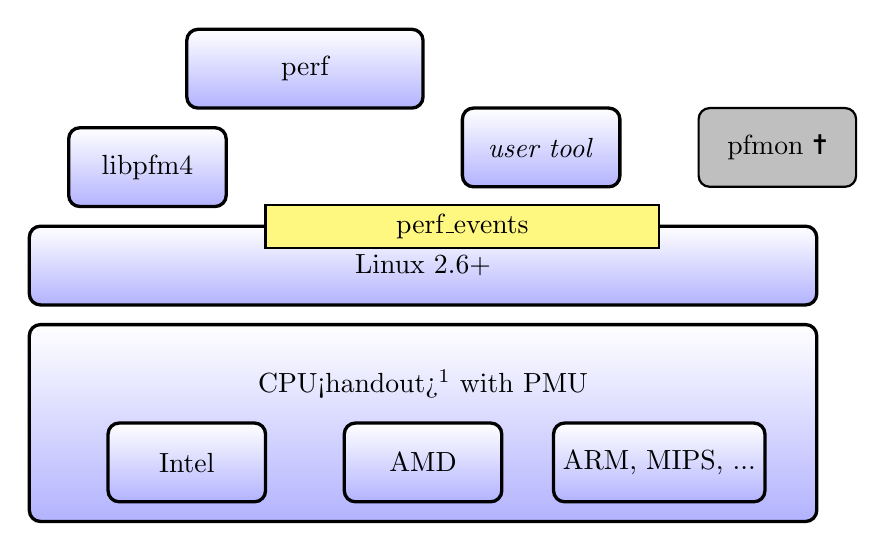
\begin{tikzpicture}[scale=1,transform shape]
\tikzstyle{size}=[minimum width=2 cm, minimum height=1 cm,anchor=center]

\tikzstyle{module}=[size,rectangle,rounded corners,draw=black, top color=white, bottom color=blue!30,very thick, text centered]
\tikzstyle{interface}=[rectangle,draw=black, fill=yellow!50,thick, text centered]
\tikzstyle{label}=[size,rectangle,text centered]

\node [module,minimum width=10 cm,minimum height=2.5 cm] at (0,0.5) (cpu)  {};
\node [label] at (0,1) (cpuLabel) {CPU\only<handout>{\footnote{detailed list: \url{http://web.eecs.utk.edu/~vweaver1/projects/perf-events/support.html}}} with PMU};
\node [module] at (-3,0) (intel)  {Intel};
\node [module] at (0,0) (amd) {AMD};
\node [module] at (3,0) (arm) {ARM, MIPS, ... };

\uncover<2->{
  \node [module,minimum width=10 cm,minimum height=1 cm] at (0,2.5) (linux)  {Linux 2.6+};
  \node [interface,minimum width=5 cm] at (0.5,3) (perf)  {perf\_events};
}

\uncover<3->{
  \node [module] at (-3.5,3.75) (libpfm4)  {libpfm4};
  \node [module,minimum width=3 cm] at (-1.5,5) (perf)  {perf};
}
\uncover<4->{
  \node [module] at (1.5,4) (user)  {\textit{user tool}};
}
\uncover<5->{
  \node [size,rectangle,rounded corners,draw,thick,fill=gray!50] at (4.5,4) (pfmon)  {pfmon \Cross};
}
\end{tikzpicture}
\end{center}

\end{frame}

\only<handout>{
\begin{frame}{architecture (2)}
\begin{description}
  \item[perf] profiler tool for Linux
  \item[perf\_events] Linux kernel Interface
  \item[libpfm4] helper library to map event\only<handout>{\footnote{an event is raised if something happens in the CPU, e.g. an instructions is executed or an branch is mispredicted}} names to event encoding
  \item[pfmon, perfmon] predecessor of perf / perf\_events , development stopped\only<handout>{\cite{pfmon2007}}
  \item[PMU] Performance Monitoring Unit, also known as Hardware Performance Counters (HPCs)\only<handout>{\cite{Azimi2009}}
  \begin{itemize}
    \item CPU registers, no overhead
    \item if configured, count performance in the CPU automatically
    \item can generate an interrupt on overflow
    \item can be read by software
  \end{itemize}
\end{description}
\end{frame}
}

\begin{frame}{perf\_events\only<handout>{\cite{kernel.org2011,Eranian2010}}}
\begin{itemize}
  \item the Linux kernel interface
  \item abstraction of hardware
  \begin{itemize}
    \item mimic Intel architected PMU
  \end{itemize}
  \pause
  \item based on file descriptors
  \begin{itemize}
    \item \code{perf\_event\_open}, \code{read}, \code{close}, \code{ioctl}
  \end{itemize}
  \pause
  \item hardware events (performance counters, ...)
  \item software events, e.g.:
  \begin{itemize}
    \item page faults
    \item context switches
  \end{itemize}
\end{itemize}
\end{frame}

\begin{frame}{perf tool\only<handout>{\cite{Eranian2010}}}
\begin{itemize}
  \item cmdline tool, curses-based gui
  \item included in kernel source tree (tools/perf)
  \item profiling support similar to Oprofile\only<handout>{\cite{oprofile}}
\only<handout>{
  \begin{itemize}
    \item collection $\Rightarrow$ perf record $\Rightarrow$ binary output file
    \item high level analysis $\Rightarrow$ perf report
    \item source level analysis $\Rightarrow$ perf annotate
    \item remote collect\only<handout>{\footnote{Collect data on an remote machine and analyze datafile locally}}, local analysis possible
  \end{itemize}
}
\end{itemize}
\pause
\begin{center}
  \includegraphics[width=11cm]{res/perfgui}
\end{center}
\end{frame}

\begin{frame}{perf events}
\begin{itemize}
\uncover<1->{
  \item software events
  \begin{itemize}
    \item pure kernel counters, e.g.: context-switches, minor-fault
  \end{itemize}
}
\uncover<2->{
  \item hardware events
  \begin{itemize}
    \item PMU, depending on hardware, e.g.: number of cycles, instructions retired
  \end{itemize}
}
\uncover<3->{
  \item tracepoint events
  \begin{itemize}
    \item based on ftrace\only<handout>{\footnote{tracing utility built directly into the Linux kernel}} infrastructure
  \end{itemize}
}
\end{itemize}
\end{frame}

\begin{frame}[fragile]{event multiplexing\only<handout>{\cite{kernel.org2011}}}
\begin{itemize}
\uncover<1->{
  \item problem: PMU only have a small number of counters
}
\uncover<2->{
  \item solution: time multiplexing
  \item[$\Rightarrow$] an event is not measured all the time and scaled at the end
  \item scaling: $final\_count = raw\_count \frac{time\_enabled}{time\_running}$
}
\end{itemize}
\pause
\begin{lstlisting}[basicstyle=\tiny\ttfamily]
perf stat -B -e cycles,cycles,cycles ./noploop 1

 Performance counter stats for './noploop 1':

    2,809,946,289 cycles                    (scaled from 74.98%)
    2,809,725,593 cycles                    (scaled from 74.98%)
    2,810,797,044 cycles                    (scaled from 74.97%)
    2,809,315,647 cycles                    (scaled from 75.09%)

       1.295007067  seconds time elapsed
\end{lstlisting}
\end{frame}

\begin{frame}[fragile]{\code{perf stat}}
\begin{itemize}
  \item aggregated counter statistics
  \item options for human readable output
  \item options for machine readable output
  \item event filtering
\end{itemize}
\pause
\begin{lstlisting}[basicstyle=\tiny\ttfamily]
perf stat -e cycles,instructions,context-switches,L1-dcache-load-misses -B dd if=/dev/urandom of=/dev/null  count=10000

 Performance counter stats for 'dd if=/dev/urandom of=/dev/null count=10000':

        1879949533 cycles                  
        4267794459 instructions             #      2.270 IPC  
               126 context-switches        
             42895 L1-dcache-load-misses   

        0.949068666  seconds time elapsed
\end{lstlisting}
\end{frame}

\begin{frame}[fragile]{\code{perf record}}
\begin{itemize}
  \item collect profiles
  \begin{itemize}
    \item per-thread
    \item per-process
    \item per-cpu
  \end{itemize}
  \item event filter
  \item call graph
  \item stores samples in binary file
\end{itemize}
\pause
\begin{lstlisting}
perf record -g -- ./test
\end{lstlisting}
\end{frame}

\begin{frame}[fragile]{\code{perf report}}
\begin{itemize}
  \item presents data from \code{perf record}
  \item different output
  \begin{itemize}
    \item console gui
    \item stdio print
    \item raw
  \end{itemize}
\pause
  \item filters 
  \begin{itemize}
    \item threads
    \item symbols
    \item shared object
  \end{itemize}
\end{itemize}
\pause
\begin{lstlisting}[basicstyle=\tiny\ttfamily]
Events: 144  cycles                                                    
+     71.21%         test  test               [.] recFib              
+     27.91%         test  test               [.] loopFib             
+      0.86%         test  [kernel.kallsyms]  [k] __kmalloc           
+      0.02%         test  [kernel.kallsyms]  [k] perf_event_comm_ctx 
+      0.00%         test  [kernel.kallsyms]  [k] native_write_msr_saf
                                                                      
Press '?' for help on key bindings                                     
\end{lstlisting}
\end{frame}

\begin{frame}[fragile]{\code{perf annotate -l}}
\begin{itemize}
  \item annotate source code
  \item data from \code{perf record}
\end{itemize}
\begin{center}
  \includegraphics[width=11cm]{res/perfannotate}
\end{center}
\end{frame}

\begin{frame}{\code{perf timechart}}
\begin{itemize}
  \item records system behavior during a workload
  \item samples data in file
  \item creates SVG picture out of the sample
\end{itemize}
\pause
\includegraphics[width=12cm]{res/timechart}
\end{frame}

\begin{frame}[fragile]{\code{perf top}}
\begin{itemize}
  \item top like program
  \item print sampled functions in real time
\end{itemize}
\pause
\begin{lstlisting}[basicstyle=\tiny\ttfamily]
   PerfTop:       2 irqs/sec  kernel: 0.0%  exact:  0.0% [1000Hz cycles],  (target_pid: 24791)
------------------------------------------------------------------------------

             samples  pcnt function                       DSO
             _______ _____ ______________________________ __________________

               43.00 21.7% malloc                         xulrunner-stub    
               38.00 19.2% pthread_mutex_lock             libpthread-2.13.so
               27.00 13.6% __pthread_mutex_unlock_usercnt libpthread-2.13.so
               22.00 11.1% free                           xulrunner-stub    
                8.00  4.0% jpeg_idct_islow                libjpeg.so.62.0.0 
                8.00  4.0% realloc                        xulrunner-stub    
                7.00  3.5% __floor                        libm-2.13.so      
                6.00  3.0% __memcpy_ssse3                 libc-2.13.so      
                5.00  2.5% __GI___strcmp_ssse3            libc-2.13.so      
\end{lstlisting}
\end{frame}

%\begin{frame}{analysis capabilities}
%How can it be used at CERN?
%How can the data be used?
%in which ways can we look at the data and how are those ways relevant or useful for software or hardware benchmarking
%\end{frame}

\begin{frame}{summary / conclusion}
\begin{itemize}
  \item summary
  \begin{itemize}
    \item find bottlenecks in software and system
    \item perf can be used in scripts
    \item or a user written tool can use perf\_events interface
    \item different use cases of perf
    \item abstraction of hardware
    \item more than hardware counters
  \end{itemize}
\pause
  \item conclusion
  \begin{itemize}
    \item looks like \textbf{the} (new) way for performance monitoring in Linux
    \item probably stable interface through hardware abstraction
    \item behavior of PMU are Manufacture specific
    \begin{itemize}
      \item[$\Rightarrow$] difficult but tempting to compare results
    \end{itemize}
  \end{itemize}
\end{itemize}
\end{frame}

\only<handout>{
\appendix

\begin{frame}{Literature}
\begin{scriptsize}
  \printbibliography
\end{scriptsize}
\end{frame}

}

\end{document}
